\documentclass[10pt,a4paper]{article}
\usepackage[utf8]{inputenc}
\usepackage[italian]{babel}
\usepackage{amsmath}
\usepackage{amsfonts}
\usepackage{amssymb}
\usepackage{graphicx}
\usepackage[left=2cm,right=2cm,top=2cm,bottom=2cm]{geometry}
\newcommand{\rem}[1]{[\emph{#1}]}

\author{Gruppo AC \\ Federico Belliardo, Francesco Mazzoncini, Giulia Franchi}
\title{Esercitazione N.2: Circuito RC - Filtri Passivi.}
\begin{document}

\maketitle

\section{Scopo e strumentazione}

Misurare la frequenza di un filtro passa-basso e studiare la variazione della risposta del filtro in funzione del carico applicato a valle. In seguito studiare la l'attenuazione di un filto passa-banda. 

\section{Filtro passa-basso}

\paragraph{Progettazione filtro.}
Si vogliono trovare i valori dei componenti resistivo e capacitivo del filtro perchè trasmetta un segnale sinusoidale di frequenza $2kHz$ e attenui il rumore a $20kHz$.

\begin{figure}[h]
\centering
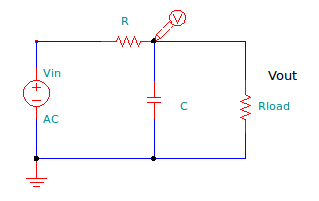
\includegraphics[scale=1.0]{passabasso.png}
\caption{Schema del circuito passa-basso}
\end{figure}

Risolvendo il circuito e chiamando $r$ la resitenza di carico e $R$ la resistenza del passabasso si ottiene la seguente relazione per il modulo dell'attenuazione:

$\vert A(\omega) \vert = \frac{1}{\sqrt{(1+x)^2+(\frac{f}{f_{0}})^2}} $. Dove $f_0$ è la frequenza di taglio del filtro. Definite $f_2 = 20 kHz$ e $f_1 = 2 kHz$ le freuenze del rumore e del segnale e $x = \frac {R}{r}$ otteniamo come rapporto di attenuazione: 
$\vert \frac{A(2 kHz)}{A(20 kHz} \vert = \sqrt{\frac{{f_0}^2 (1+x)^2 + {f_2}^2}{{f_0}^2 (1+x)^2 + {f_1}^2}}$

Selezionando una resistenza $R = 1 k\Omega$ del filtro molto minore del carico $r = 100 k\Omega$ otteniamo $x = 0.01$ cioè un valore per $x$ trascurabile e possiamo scrivere (le unità sono state prese $kHz$): 
$\vert \frac{A(2 kHz)}{A(20 kHz} \vert = \sqrt{\frac{{f_0}^2  + 400}{{f_0}^2 + 4}}$. Si sceglierà la frequenza di taglio del filtro essere $f_0 = 2kHz$. Con un condensatore $C = 80 nF$ si ottiene una rapporto segnale rumore $\vert \frac{A(2 kHz)}{A(20 kHz} \vert \sim 7$ e una attenuazione del segnale $\vert A(2 kHz) \vert \sim \frac{1}{\sqrt{2}}$.

Abbiamo a disposizione un condensatore da $C = (70 \pm 3) \, nF$, e questo implica avere una resistenza $R = (1.20 \pm 0.01) \, k\Omega$.
La frequenza di taglio quindi è $f_0 = (1.90 \pm 0.01) \, kHz$ e da questi valori stimiamo i valori di $\vert A(2 kHz) \vert = 0.69 \pm 0.02 $ e di $\vert \frac{A(2 kHz)}{A(20 kHz} \vert = 7.3 \pm 0.1$.

\paragraph{Misura frequenza di taglio.}
Abbiamo preso varie misure del segnale con frequenze comprese tra $100Hz$ e $1MHz$, riportiamo i dati relativi nella tabella.

\begin{table}[h]
\centering
\begin{tabular}{|c|c|c|c|}
\hline 
$V_{out} (V)$  &  $\sigma V_{out} (V)$ &  $f(kHZ)$ & $\sigma f(kHz)$ \\ 
\hline 
5.2 & 0.2 & 0.100 & 0.001 \\ 
\hline 
5.2 & 0.2 & 0.200 & 0.002 \\ 
\hline 
4.9 & 0.2 & 0.500 & 0.005 \\ 
\hline 
4.6 & 0.1 & 1.01 & 0.01 \\ 
\hline 
4.1 & 0.2 & 1.50 & 0.02 \\ 
\hline 
3.5 & 0.1 & 2.00 & 0.02 \\ 
\hline 
2.7 & 0.1 & 3.00 & 0.03 \\ 
\hline 
2.2 & 0.1 & 4.00 & 0.04 \\ 
\hline 
1.75 & 0.07 & 5.00 & 0.05 \\ 
\hline 
1.13 & 0.05 & 8.00 & 0.08 \\ 
\hline 
0.92 & 0.05 & 10.1 & 0.1 \\ 
\hline 
0.164 & 0.005 & 67.0 & 0.7 \\ 
\hline 
0.136 & 0.005 & 84.0 & 0.8 \\ 
\hline 
0.090 & 0.005 & 84.0 & 0.8 \\ 
\hline 
0.090 & 0.005 & 110.0 & 0.1 \\ 
\hline 
0.074 & 0.005 & 139.0 & 0.1 \\ 
\hline 
0.068 & 0.005 & 156.0 & 0.2 \\ 
\hline 
0.064 & 0.005 & 165.0 & 0.3 \\ 
\hline 
\end{tabular} 
\caption{Dati tensioni filtro passa-basso.}
\end{table}

Abbiamo eseguit 3 fit numerici:\\
\begin{itemize}
\item
Fit numerico con una costante per il range di frequenze in cui il filtro passabasso non attenua il segnale in entrata. 
La retta ottenuta come da aspettativa è concorde con $0\,dB$, $A = (0.22 \pm 0.1) \, dB$ entro $3\sigma$. Come è evidente dal grafico il $\chi^2$ risulta essere molto piccolo: $\chi^2/ndof = 0.82/2$.

\begin{figure}[h]
\centering
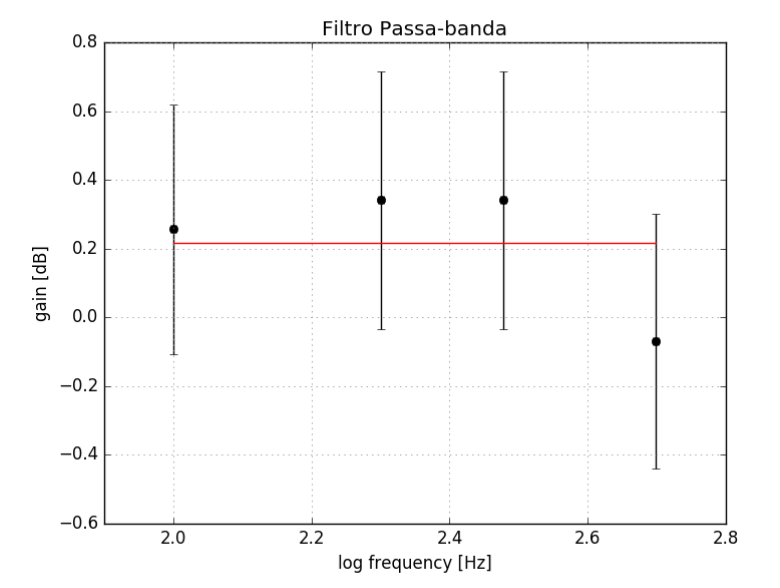
\includegraphics[scale=0.4]{immagine1.png}
\caption{Fit orizzontale}
\end{figure}

\item
Fit con una retta a due parametri: $y = mx + q$ per il range di frequenze in cui il filtro passabasso attenua il segnale in entrata, ottenendo: $m = (-21 \pm 2) \, \frac{dB}{decade}$ e $q = (7 \pm 1) \cdot 10 \, dB$, con la seguente matrice di covarianza:
$\left(\begin{array}{cc}
4.9 & -24.8 \\ 
-24.8 & 125
\end{array}\right)$

\begin{figure}[h]
\centering
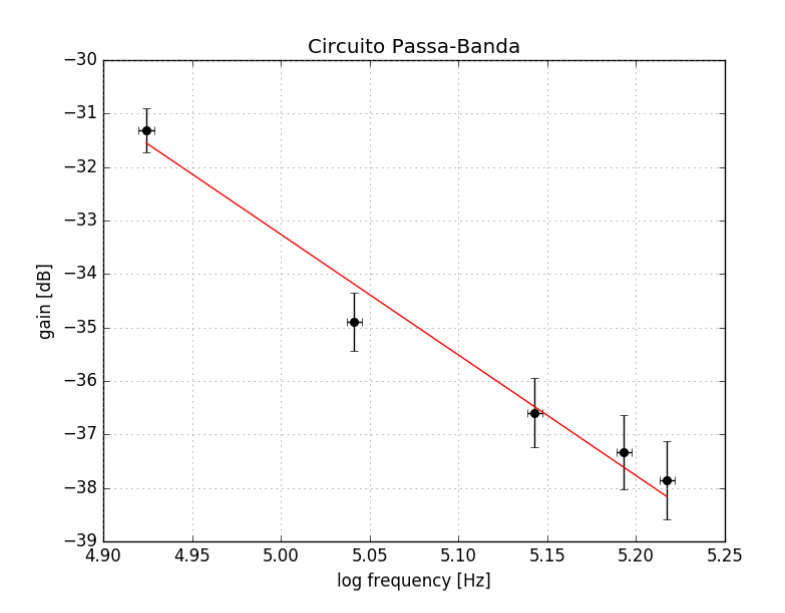
\includegraphics[scale=0.4]{immagine2.png}
\caption{Fit orizzontale}
\end{figure}

Si è misurata la frequenza di taglio dall'intersezione delle due rette del fit. Chiamate le rette $y = a_1 x+b_1$ e $y = a_2 x+b_2$, il loro punto di intersezione è $f_0 = \frac{b_1 - b_2}{a_2 - a_1}$. Se abbiamo $a_1 = 0$ allora otteniamo: $f_0 =  \frac{b_1 - b_2}{a_2}$ e da questo $f_{0} = (2.5 \pm 1.0) \, kHz$. 

\item
Fit numerico su tutti i dati con la funzione di trasferimento: $\vert A(f) \vert = \frac{1}{\sqrt{(\frac{f}{f_0})^2}}$, ottenendo: $f_t = (196 \pm 1) \cdot 10 \, Hz$, con $\chi^2/ndof = 0.15$.

\end{itemize}

\paragraph{Impedenza del circuito a bassa frequenza.}
L'impedenza di ingresso di un circuito come quello disegnatio all'inizio della relazione è $Z_{ingresso} = R+\frac{r}{j \omega C r+1}$ , dunque a bassa frequenza in condensatore è un aperto dunque l'impedenza di ingresso è $R+r$, mentre ad alta frequenza è un cortocircuito dunque l'impendenza è $R$. Alla frequenza di taglio abbiamo poi: $Z_{ingresso} = R + \frac{Rr}{jr+R}$. L'efetto della resistenza di carico sul circuito è di diminuirne il guadagno, secondo la formula: $\vert A(\omega) \vert = \frac{1}{\sqrt{(1+x)^2+(\frac{f}{f_{0}})^2}} $.
Lo scostamento della risposta da quella del filtro ideale è tanto maggiore quanto il carico resistivo è più vicino alla resistenza del filto.

\section{Filtro passa-banda}

\begin{figure}[h]
\centering
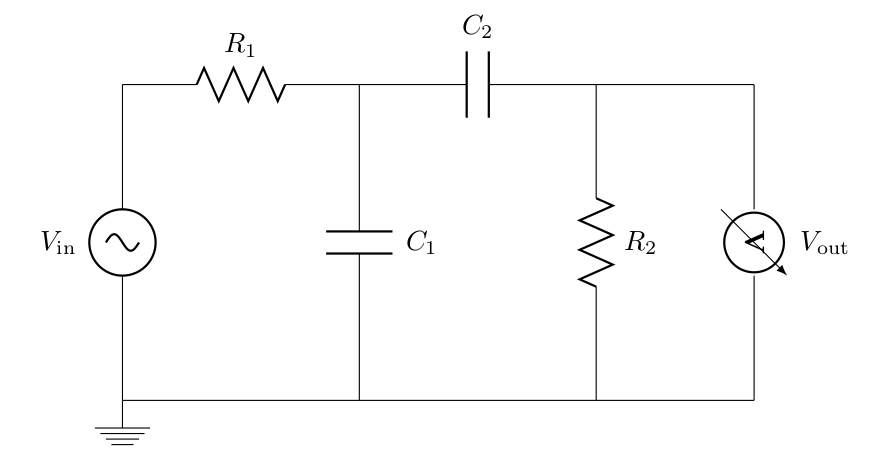
\includegraphics[scale=0.4]{passabanda.png}
\caption{Filtro passa banda}
\end{figure}

\paragraph{Verifiche sui circuiti passa alto e passa basso.}
I valori teorici delle frequenze per i filtri passa-basso e passa-alto utilizzati in questa esperienza sono riportate nella tabella seguente insieme ai valori di condensatori e resistenze:

\begin{figure}[h]
\centering
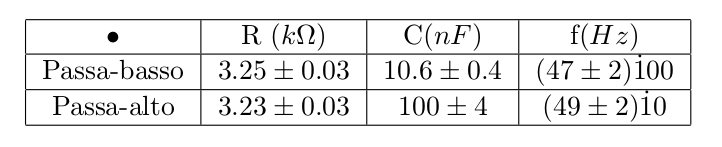
\includegraphics[scale=0.4]{tabella2.png}
\caption{Filtro passa banda}
\end{figure}

Il seguente grafico riporta i dati del filtro passa-banda:

\begin{figure}[h]
\centering
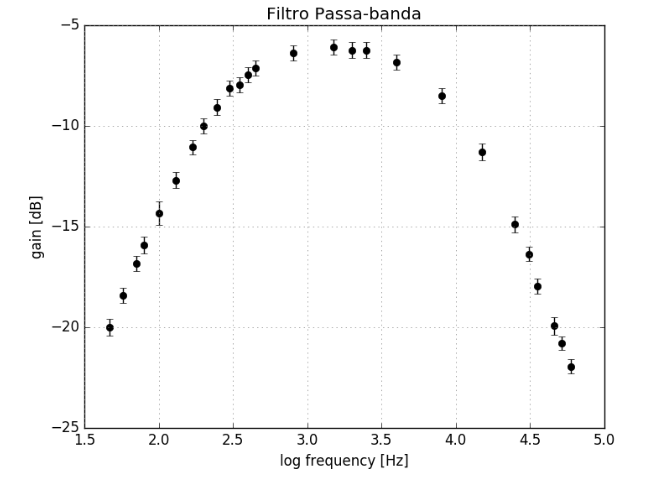
\includegraphics[scale=0.4]{immagine5.png}
\caption{Filtro passa banda}
\end{figure}

\paragraph{Misure sul fitro passa banda.}
La tabella riporta le misure di tensione in uscita per varie frequenze del passabanda.


\begin{table}[h]
\centering
\begin{tabular}{|c|c|c|c|c|c|}
\hline 
$V_{out}$ & $\sigma V_{out}$ & $f(kHZ)$ & $\sigma f(kHz)$ \\ 
\hline 
0.50 & 0.02 & 0.0467 & 0.0005 \\ 
\hline 
0.60 & 0.02 & 0.0574 & 0.0006 \\ 
\hline 
0.72 & 0.02 & 0.0704 & 0.0007 \\ 
\hline 
0.80 & 0.03 & 0.0800 & 0.0008 \\ 
\hline 
0.96 & 0.06 & 0.100 & 0.001 \\ 
\hline 
1.16 & 0.04 & 0.130 & 0.001 \\ 
\hline 
1.40 & 0.04 & 0.170 & 0.002 \\ 
\hline 
1.58 & 0.05 & 0.200 & 0.002 \\ 
\hline 
1.76 & 0.06 & 0.247 & 0.002 \\ 
\hline 
1.96 & 0.06 & 0.300 & 0.003 \\ 
\hline 
2.00 & 0.06 & 0.352 & 0.004 \\ 
\hline 
2.12 & 0.07 & 0.400 & 0.004 \\ 
\hline 
2.20 & 0.07 & 0.449 & 0.004 \\ 
\hline 
2.40 & 0.07 & 0.800 & 0.008 \\ 
\hline 
2.48 & 0.08 & 1.50 & 0.2 \\ 
\hline 
2.44 & 0.08 & 2.20 & 0.3 \\ 
\hline 
2.44 & 0.08 & 2.50 & 0.3 \\ 
\hline 
2.28 & 0.07 & 4.00 & 0.4 \\ 
\hline 
1.88 & 0.06 & 8.00 & 0.8 \\ 
\hline 
1.36 & 0.05 & 15.0 & 0.2 \\ 
\hline 
0.90 & 0.03 & 25.0 & 0.3 \\ 
\hline 
0.76 & 0.02 & 30.9 & 0.4 \\ 
\hline 
0.63 & 0.02 & 35.5 & 0.5 \\ 
\hline 
0.50 & 0.02 & 45.6 & 0.5 \\ 
\hline 
0.45 & 0.01 & 51.3 & 0.5 \\ 
\hline 
0.40 & 0.01 & 59.3 & 0.6 \\ 
\hline 
\end{tabular} 
\caption{Dati tensioni filtro passa-banda.}
\end{table}



Sono stati eseguiti fit lineari con la funzione \emph{curvefit} della libreria \emph{pylab}, in cui abbiamo impostato il parametro \emph{absolute sigma = "true"}. Per la parte centrale è stata fittata solo una costante. I parametri ottenuti e i relativi $\chi^2$ e matrici di covarianza sono:

\begin{itemize}
\item \textbf{Basse frequenze}\\
$ m = (17 \pm 2) \, \frac{dB}{decade}$ e $q = (50 \pm 3) \, dB$. La matrice di covarianza è: 
$\left(\begin{array}{cc}
3.58 & -6.53 \\ 
-6.53 & 11.9
\end{array} \right)$

\begin{figure}[h]
\centering
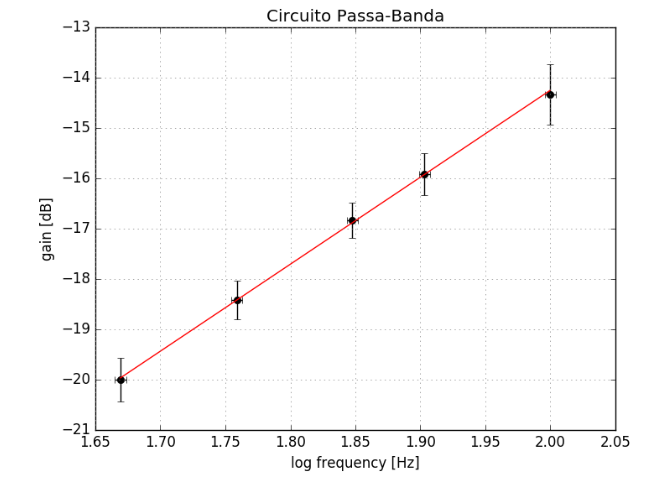
\includegraphics[scale=0.4]{immagine6.png}
\caption{Filtro passa banda - Salita}
\end{figure}

\item \textbf{Guadagno massimo}\\
$q = (-6.2 \pm 0.4) \, dB$. Il gaudagno massimo è compatibile con $-6 \, dB$ come atteso teoricamente.

\begin{figure}[h]
\centering
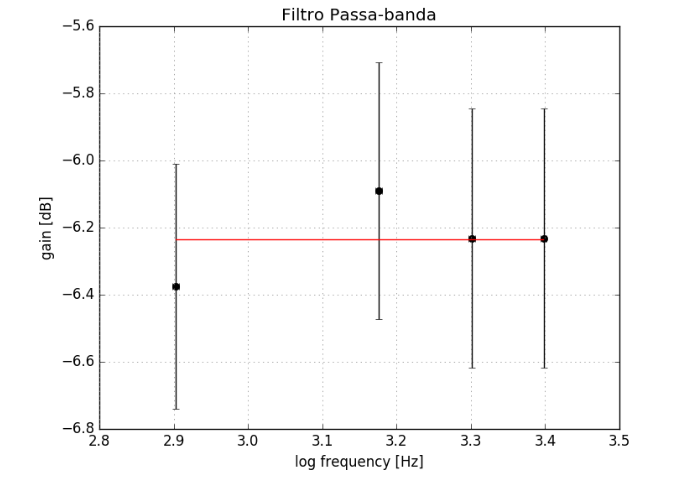
\includegraphics[scale=0.4]{immagine7.png}
\caption{Filtro passa banda - Guadagno massimo}
\end{figure}

\item \textbf{Alte frequenze}
$m = (-19 \pm 2) \, \frac{dB}{decade}$, $q = (70 \pm 7) \, dB$. La matrice di covarianza che si ottiene è:
$\left(\begin{array}{cc}
2.35 & -10.5 \\ 
-10.5 & 48.6
\end{array}\right)$

\begin{figure}[h]
\centering
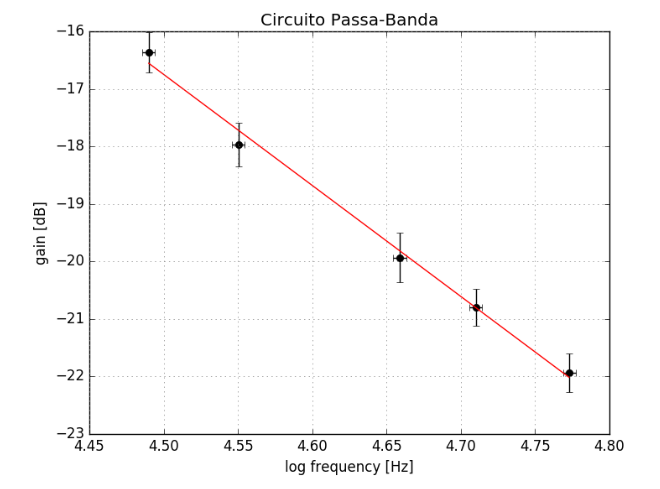
\includegraphics[scale=0.4]{immagine9.png}
\caption{Filtro passa banda - Discesa}
\end{figure}

\end{itemize} 

I valori delle frequenze di taglio (alta e bassa calcolate intersecando le due rette e propagando opportunamnte gli errori sono: 
$f_1 = (9\pm1) \, kHz$ e $f_2 = (25 \pm 5) \cdot 10 Hz$. Queste misure sono compatibili rispettivamente con il doppio e un mezzo delle misure sul passa-basso e passa-alto presi singolarmente.


\paragraph{Spiegazioni teoriche.}
La funzione di trasferimento teorica per un circuito passa banda come quelli disegnati sopra è: 
$V_{out} = A_{1} A_{2} \frac{Z_{in}^2}{Z_{out}^2+Z_{in}^2} V_{in}$, dove gli apici si riferiscono a al primo o al secondo circuito in sequenza. 

La seguente tabella riassume le impedenze di ingresso e sucita per circuiti passa basso:

\begin{table}[h]
\centering
\begin{tabular}{|c|c|c|}
\hline 
 & Passa-basso  & Passa-alto \\
\hline 
Ingresso & $R+\frac{1}{j \omega C}$ & $R+\frac{1}{j \omega C}$\\ 
Uscita & $AR$ & $j \omega C A$\\
\hline 
\end{tabular} 
\caption{Riassunto resistenze di ingresso e di uscita.}
\end{table}


Semplificando l'espressione otteniamo: $V_{out} = A_{1} A_{2} \frac{1}{1+\frac{R_1}{R_2} A_1 A_2} V_{in}$.
E nel nostro caso (due resistenze uguali otteniamo:
$V_{out} = A_{1} A_{2} \frac{1}{1+A_1 A_2} V_{in}$, che è limitato dall'alto da $A_{max} = \frac{1}{2}$.
Se chiamiamo $\omega_1$ la frequenza di taglio del circuito passa alto e $\omega_2$ la frequenza di taglio del circuito passa alto e la frequenza del cicruito passa basso otteniamo i seguenti limiti per l'attenuazione:

\begin{itemize}
\item $\omega \ll \omega_1$ allora $A_1 \sim 1$ dunque 
$A_{tot} = \frac{A_2}{1+A_2}$, sviluppando otteniamo 
$A_{tot} = \frac{1}{2} \frac{1}{1-j \frac{\frac{\omega_2}{2}}{\omega}}$ dunque il filtro è equivalente a un passa alto con frequenza di taglio $\frac{\omega_2}{2}$. 
\item $\omega \gg \omega_2$ allora $A_2 \sim 1$ dunque 
$A_{tot} = \frac{A_1}{1+A_1}$, sviluppando otteniamo:
$A_{tot} = \frac{1}{2} \frac{1}{1+j \frac{omega}{2 \omega_1}}$.
\end{itemize}

Se vogliamo che $A_{tot} = A_1 A_2$ deve essere $R_1 \ll R_2$ come è evidente.

\section{Conclusioni e osservazioni}
Abbiamo acquisito tutte le misure controlando che l'ampiezza di ingresso rimanese costante a $V_{in} = 5 \, V$, in accoppiamento AC, per eseguire le misure agli estremi dell'intervallo di frequenze sarebbe stato conveniente aumentare l'ampiezza del voltaggio in ingresso, per rendere meno influente il rumore ad alta frequenza. Un voltaggio di ingresso di $V_{in} = 30 \, V$ sarebbe stato più appropriato. L'altissimo errore sulle misure di frequenza ottenute con l'intersezione fra le rette è dovuto al fatto che l'errore sul coeffiente angolare è fortemente dipendente dall'errore sulle ordinate delle misure e essendo la scala di fequenza logaritmica l'errore viene amplificato esponenzialmente. E' da notare che che l'errore sulle ampiezze è stato evidentemente sovrastimato, come si vede dal fatto che i $\chi^2$ vengono sistematicamente inferiori di quelli attesi. Infatti sui voltaggi si è sempre considerato un errore del $3\%$.

\end{document} 